\subsubsection{27.12.14}
\begin{enumerate}
	
	\item Time of beginning and ending of meeting: 16:15 - 20:00.
	
	\item Purposes of meeting: 
	\begin{enumerate}
		
		\item To finish soldering wires.
		
		\item To elaborate MCB that can to keep rolling goal when power off.
		
        \item To write more comfortable programme of control robot.
		
	\end{enumerate}

	\item Work that has been done:
	\begin{enumerate}
		
		\item Ends of all wires were soldered.
		
		\item It was decided to install on MCB two stickers so that MCB doesn't open due to weight of rolling goal when robot is on the ramp. Stickers were installed but didn't tested because we hasn't got original rolling goals.
		
		\begin{figure}[H]
			\begin{minipage}[h]{0.1\linewidth}
				\center  
			\end{minipage}
			\hfill
			\begin{minipage}[h]{0.29\linewidth}
				\center{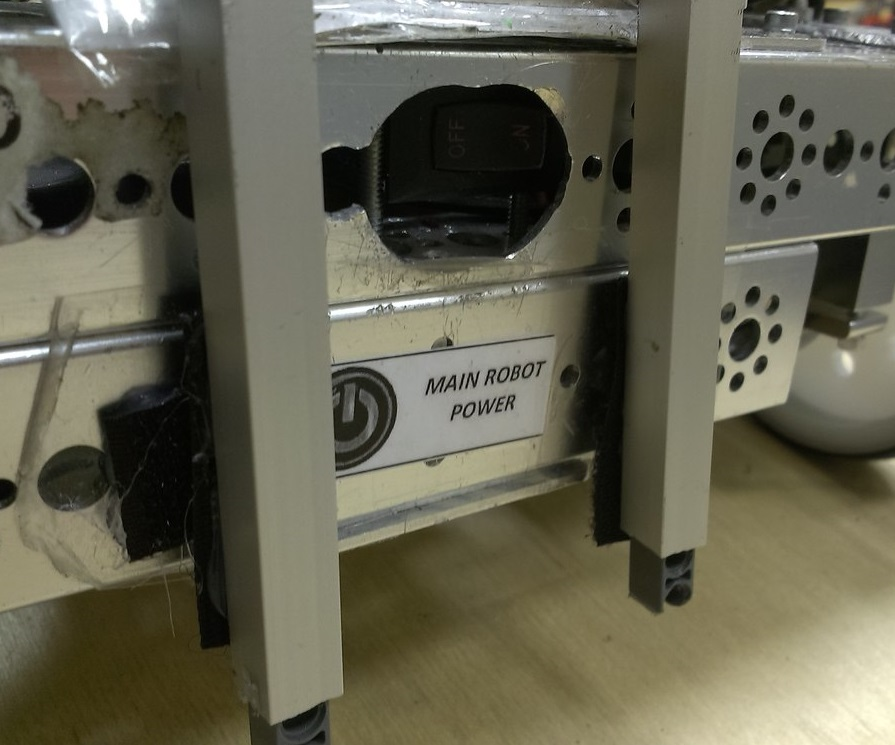
\includegraphics[scale=0.2]{days/27.12.14/images/01}}
			\end{minipage}
			\hfill
			\begin{minipage}[h]{0.29\linewidth}
				\center{
\includegraphics[scale=0.2]{days/27.12.14/images/02}}
			\end{minipage}
			\hfill
			\begin{minipage}[h]{0.1\linewidth}
				\center  
			\end{minipage}
			\caption{Stickers on MCB}
		\end{figure}
		
        \item It was wrote more comfortable programme of control robot. Now control of moving is by multi positional button "TopHat". Robot can move by 8 ways: forward, backward, clockwise rotation, counterclockwise rotation and turning by only one pair of wheels (left or right). Also robot moves slower when operator presses button №7.
        \begin{figure}[H]
	  	  \begin{minipage}[h]{0.2\linewidth}
	  		\center  
	  	  \end{minipage}
	  	  \begin{minipage}[h]{0.6\linewidth}
	  		\center{
\includegraphics[scale=0.3]{days/27.12.14/images/03}}
	  		\caption{The scheme of control moving}
	  	  \end{minipage}
	   \end{figure}
	   
	   \item During the tests of programme it was found that repaired motor doesn't work on the field. It works when robot above the floor but doesn't work under the load. It was found that the problem is in the motor and not in the driver or wire. We need to replace it.
	   
	\end{enumerate}
	
	\item Results:
	\begin{enumerate}
		
		\item Ends of all wires were soldered.
		
		\item MCB was improved but wasn't tested.
		
        \item New programme of control robot was tested. Result positive.
		
	\end{enumerate}
	
	\item Tasks for the next meetings:
	\begin{enumerate}
		
		\item To replace broken motor.
		
		\item To replace broken slat.
			
	\end{enumerate}
\end{enumerate}
\fillpage
